\section{The Framework}

Based on the empirical finding that a teen posts more stressful posts per day
during stressor-event periods than non-stressor-event periods (referred to as \emph{stressful posting} rate),
we present a statistic model of teen's stressful posting rate.
With the model, we can extract stressful periods
and stressor events to be extracted from each stressful period.

\subsection{A Statistic Model of Teens Stressful Period}

\subsubsection{Poisson Process of Stressful Posting Rates Over a Time Period}

We model teen's posting behaviors during stressor-event and non-stressor-event periods as two independent homogeneous Poisson processes.
The number of stressful posts created during a stressor-event period is modeled as a
a homogeneous Poisson process of stressful posting rate $\lambda_1$ per unit time (say, per day), and
the number of stressful posts created during a non-stressor-event period as another
independent homogeneous Poisson process of stressful posting rate $\lambda_0$ per unit time.
From Fig.~\ref{fig:ratioGrade}, we observe that $\lambda_1 > \lambda_0$.

In general, for a Poisson process of a constant stressful posting rate $\lambda$,
the number of stressful posts $N$ posted during a period of length $T$
(which needs not to be contiguous) is a Poisson random variable with mean $\lambda \times T$.
That is, the probability that a teen posts $n$ stressful posts within $T$ time units can be computed as:
$Pr[N=n|\lambda]=\frac{e^{-\lambda T}{(\lambda T)}^n}{n!}$, where $n=0,1,\cdots,\infty$.
Under the Poisson process model, the number of stressful posts created by a teen in non-overlapping time periods are
independent random variables.

\subsubsection{Inferring Stressful Periods From Stressful Posting Rates}

To measure the confidence that a teen has a higher stressful posting rate
during stressor-event periods than non-stressor-event periods, %thus the likelihood of a resulted stressful period,
we use teens historic posting information to estimate the probability distributions of the
stressful posting rates $\lambda_1$ and $\lambda_0$, and then compute a statistic
based on these posterior distributions.  This statistic is our metric for stressor-event periods, i.e.,
stressful periods.

Let $N_1$ be the number of stressful posts during stressor-event periods of length $T_1$,
and $N_0$ be the number of stressful posts during non-stressor-event periods of length $T_0$.
In estimation theory, $N_1$ and $N_0$ are minimal sufficient statistics for estimation of
$\lambda_1$ and $\lambda_0$, respectively.
Assume a Jeffreys non-informative prior on the stressful posting rate $\lambda_1$ and $\lambda_0$~\cite{Jeffrey}.
That is, for $\lambda_1,\lambda_0 > 0$, the prior density
$p(\lambda_1,\lambda_0) \propto \frac{1}{\sqrt{\lambda_1 \lambda_0}}$,
and the corresponding priors are
$p(\lambda_1) \propto \frac{1}{\sqrt{\lambda_1}}$ and
$p(\lambda_0) \propto \frac{1}{\sqrt{\lambda_0}}$.
According to the Bayes Rule, the posterior distribution of $\lambda_i$ (for $i$=0,1) is
{\small
\begin{flalign}
\begin{split}
&p(\lambda_i|N_i) \propto Pr[N_i|\lambda_i] p(\lambda_i)=(\frac{1}{\sqrt{\lambda_1\lambda_0}}\times \frac{e^{-\lambda_i T_i}{(\lambda_i T_i)}^{N_i}}{N_i!} \times \frac{1}{\sqrt{\lambda_i}})\\
&\propto \lambda_i^{N_i^{-0.5} e^{-T_i \lambda_i}}\\
\end{split}
\end{flalign}
}

Normalizing the posteriors into 1, we have
{\small
\begin{equation}
p(\lambda_i=x|N_i) = \left\{ \begin{array}{ll}
\frac{T_i{(T_ix)}^{N_i^{-0.5}e^{-T_ix}}}{\gamma(N_i+0.5)} & \mbox{if $x$ $\geq$ 0}, \\
0   & \mbox{otherwise}
\end{array}
\right.
\end{equation}
}
where $\gamma(z)=\int_0^{\infty}t^{z-1}e^{-t}~dt$ is the gamma function.

We quantify the probability that a teen is undergoing a stressor-event period as:
\begin{flalign}
\begin{split}
&p(\lambda_1 > \lambda_0|N_1,N_0) \\
&=\iint_{x>y}p(\lambda_1=x|N_1)~p(\lambda_0=y|N_0)~dx~dy\\
&=\iint_{x>y}\frac{T_1{(T_1x)}^{N_1^{-0.5}e^{-T_1x}}}{\gamma(N_1+0.5)}\times\frac{T_0{(T_0y)}^{N_0^{-0.5}e^{-T_0y}}}{\gamma(N_0+0.5)}~dx~dy
\end{split}
\end{flalign}

When $p(\lambda_1 > \lambda_0|N_1,N_0)$ is over a threshold $\tau$,
we are confident enough that the teen's stressful posting rate during stressor-event periods
is larger than that during non-stressor-event periods. We thus declare that the
corresponding period is a \emph{stressful period}.

\subsection{Discovery of Teens Stressful Periods}

With the model, we can now formally define and extract stressful periods.

\subsubsection{Definitions of Stressful Periods}

Assume a teen posts a list of posts $w_1,w_2,\cdots,w_m$
chronologically at time $t_1,t_2,\cdots,t_m$ on the microblog, respectively, denoted as
$W[t_1,t_m]$=$\{(t_1,w_1),(t_2,w_2),\cdots,(t_m,w_m)\}$.
From each individual post $w_i$
($1 \leq i \leq m$), teen's stress categories
$C_i$ $\subset$ ${\cal C}$
and stress level $l_i \in {\cal L}$ are detected, denoted as
\textbf{$tSW[t_1,t_m]$=$\{(t_1,C_1,l_1), (t_2,C_2,l_2), \cdots,$ $(t_m,C_m,l_m)\}$}.
Assume during [$t_1,t_m$] there are $z \in \mathbb{Z}$ unit time intervals (say, $day$)
$T_1,T_2,\cdots,T_z$.
We collapse the \emph{point-wise stress representation} $tSW[t_1,t_m]$ of
$W[t_1,t_m]$
into \emph{interval-wise representation} $TSW[T_1,T_z]=\{(T_1,n_{T_1}), (T_2,n_{T_2}), \cdots, (T_z,n_{T_z})\}$, where
$n_{T_i}$ is the aggregate number of stressful posts in the $i$-th unit time interval $T_i$ (for $1 \leq i \leq z$).
When no stressful posts are detected in $T_i$, $n_{T_i}=0$.

\begin{definition}
$TSW[T_1,T_z]$ is a \textbf{stress wave}, if
there is at least one stressful post in every unit time interval throughout [$T_1,T_z$], i.e.,
$\forall i (1 \leq i \leq z) ~(n_{T_i}>0)$.
$TSW[T_1,T_z]$ is a \textbf{big stress wave}, if it is a stress wave, and meanwhile
the probability that \emph{the stressful posting rate $\lambda_1$ during [$T_1,T_z$]
is bigger than $\lambda_0$ during historic non-stressor-event periods}
is over a confidence threshold $\tau$.
If a stress wave is not a big stress wave, then it is a
\textbf{small stress wave}.
\boxend
\end{definition}

\begin{figure}
\centering
\includegraphics[width=\linewidth,height=3cm]{figs/stressPeriod.eps}
\caption{Illustration of 4 big stress waves (A,D,E,F), 2 small stress waves (B,C), and 3 maximal stressful periods}
\label{fig:stressPeriod}
\end{figure}

Fig.~\ref{fig:stressPeriod} shows six big stress waves $A,D,E,F$ and two small waves $B,C$.
Although $B,C$ are not prominent and counted as big stress waves, they could be some
late-time oscillations of big stress wave $A$ or prelude of big stress wave $D$,
caused by the same stressor event(s).
Also, big stress wave $D$ and $E$ may arise due to the same stressor event(s).
To deal with such intermittence and continuous characteristics of teens stress
and restore an integral stressful period triggered by the same stressor event(s),
we merge these semantically related waves together
based on common stress categories.

Given $tSW[t_1,t_m]$=$\{(t_1,C_1,l_1),\cdots,(t_m,C_m,l_m)\}$,
we define the proportion of stress category $c \in {\cal C}$ in $tSW[t_1,t_m]$
over the period [$t_1,t_m$] as
{\small
\begin{equation}
cRatio(tSW[t_1,t_m],c)= \frac{|\{C_i | i \in [1,m] \wedge (c \in C_i)\}|}{\sum_{i \in [1,m]} |C_i|}
\end{equation}
}
Extending the single time period parameter of the function to allow multiple time periods,
we have
{\small
\begin{flalign}
\begin{split}
&cRatio(tSW[t_1,t_{m_1}], \cdots, tSW[t_k,t_{m_k}],c) \\
&=\frac{|\{C_i|i \in ([t_1,t_{m_1}]\cup\cdots\cup [t_k,t_{m_k}]) \wedge (c \in C_i)\}|}
{\sum_{i \in [t_1,t_{m_1}]\cup\cdots\cup [t_k,t_{m_k}]} |C_i|},\\
&\sum_{c \in {\cal C}} cRatio(tSW[t_1,t_m],\cdots,tSW[t_k,t_{m,k}],c)=1
\end{split}
\end{flalign}
}

\begin{definition}
Let $TSW[T_1,T_z]$ and $TSW'[T_1',T_z']$ be two stress waves, whose
point-wise stress representation are $tSW[t_1,t_m]$ and $tSW'[t_1',t_m']$. We call
$TSW[T_1,T_z]$ and $TSW'[T_1',T_z']$
\textbf{category distribution similar}, if and only if the Euclidean Distance of their
category distributions {\small $cDist(.) \leq \beta$},
where $\beta$ is set to 0.2 in the study, and
{\scriptsize
\begin{flalign}
\begin{split}
& cDist(tSW[t_1,t_m],tSW'[t_1',t_m'])\\
&=\sqrt{{\sum_{c \in {\cal C}}{(cRatio(tSW[t_1,t_m],c)-cRatio(tSW'[t_1',t_m'],c))}^2}}
\end{split}
\end{flalign}
}
\end{definition}

Assume from a sequence of teen's intermittent posts created throughout [$T_1,T_z$], a sequence of big stress waves $B$
and small stress waves $S$
are detected.
We call $TSW[T_1,T_z]$ a \textbf{stressful period}, if and only if the following four conditions hold.\\
\begin{itemize}
\item \textbf{\romannumeral1)} There is at least one stressful post in the start interval $T_1$ and end $T_z$.
\item \textbf{\romannumeral2)} Every two big stress waves in $B$ are category distribution similar.
\item \textbf{\romannumeral3)} The category distribution of each small wave in $S$ is similar to the \emph{centroid} category distribution of the big waves covering all the big wave time periods $[t_1,t_{m_1}], \cdots, [t_k,t_{m_k}]$ based on the extended ratio function $cRatio(tSW[t_1,t_{m_1}], \cdots, tSW[t_k,t_{m_k}],c)$, where $c \in {\cal C}$.
\item \textbf{\romannumeral4)} The probability that \emph{the stressful posting rate $\lambda_1$ throughout} [$T_1,T_z$] \emph{is bigger than $\lambda_0$ during historic non-stressor-event periods} is over a confidence threshold $\tau$.
\end{itemize}

We call $TSW[T_1,T_z]$ a \textbf{maximal stressful period}, if and only if it
is a stressful period, and there exists none stressful period $TSW[T_x,T_y]$, whose time period encloses
$[T_1,T_z]$, i.e., ($T_x \leq T_1$) $\wedge$ ($T_y \geq T_z$).
According to the definition, a big stress wave is also a stressful period.
Among the six stress waves in Fig.~\ref{fig:stressPeriod}, $(A,B)$, $(C,D,E)$, and $(F)$ form three maximal stressful periods.

\subsubsection{Method of Maximal Stressful Periods Extraction}

Discovery of maximal stressful periods proceeds in three steps:

\textbf{Step 1}: Identify all the big stress waves $B$ and small stress waves that exist in the detected stress list.
According to the definition of stressful period, each big stress wave in $B$ is a stressful period.
Let $SP$ be a set of stressful periods.
Initially, $SP$=$B$.

\textbf{Step 2:} Merge precedent or successive neighbouring small stress waves with each big stress wave $b$ in $SP$,
if the result is also a stressful period.
Each time we probe the merging, starting from the neighbour with the more similar
topic distribution as $b$. We repeat step 2 until the obtained stressful period cannot be longer.
We drop $b$ out of $SP$, and put the obtained longer stressful period into $SP$.

\textbf{Step 3:} Combine every two neighbouring stressful periods (without small stress wave gaps in between) in $SP$
if the result also constitutes a stressful period as well.
The procedure is the same as Step 2.
We repeat Step 3 until no more combination is possible.
We eliminate those successfully combined stressful periods from $SP$ and
put the obtained longer stressful period into $SP$.
The result $SP$ keeps all the maximal stressful periods.


\subsection{Extraction of Stressor Events from Maximal Stressful Periods}


\subsubsection{Definition of Stressor Events}

A stressor event $se$ is of the form
\texttt{[Dimension, Event-type, Event-instance (description, doer, act, object, time, location)}, \texttt{influence]},
Element \texttt{doer, act, object, time}, or \texttt{location} could be empty.
Table~\ref{tab:stressorEvents} gives different event types in each of the five dimensions -
\emph{school life, family life, peer relation, self-cognition,}
and \emph{romantic relation}.
Event-instance refers to the happening of a specific event with the involved doer, act, object, time, location,
and a detailed linguistic description.
%For example, an event instance description (``\emph{I have a lot of homework this weekend.}")
%tells the involved role (``\emph{I}"), act (``\emph{have}"), object (``\emph{homework}"), and time (``\emph{this weekend}")
%of an event instance, whose event type is ``\emph{having too much homework}"
%in the dimension (\emph{school life}).
An example of two stressor events of type ``\emph{having too much homework}"
and type ``\emph{feel tired of study}" in the ``\emph{school life}" dimension
is illustrated in Fig.~\ref{fig:stressorEventHierarchy}.
\begin{figure}
\centering
\includegraphics[width=\linewidth,height=3cm]{figs/stressorEventHierarchy.eps}
\caption{Example of stressor events.}
\label{fig:stressorEventHierarchy}
\end{figure}

As multiple event instances could be extracted through linguistic analysis during the teen's stressful period,
we rank them based on their \emph{stress influence}. Considering that
a stressor event usually stimulates the increase of stress levels, the higher the stress level increases, and the higher
the impact is. We measure the stress influence of the event as
%{\footnotesize
%$influence=$\\
%$w_1*\frac{level(se)}{arg~ max_{se^* \in SE} ~level(se^*)}+w_2*\frac{increase(se)}{arg~ max_{se^* \in SE} ~increase(se^*)}$
%}
{\small
\begin{flalign}
\begin{split}
influence=w_1*\frac{level(se)}{arg~ max_{se^* \in SE} ~level(se^*)}\\
+w_2*\frac{increase(se)}{arg~ max_{se^* \in SE} ~increase(se^*)}
\end{split}
\end{flalign}
}
where
1) $level(se)$: the accumulated stress level in the time unit when the event's influence starts;
To identify the event's starting time, we look for linguistic words/phases that indicate time
(e.g., exact date, \emph{today, tomorrow, yesterday, the day after tomorrow, on the weekend,} etc.).
When no such words are found or the starting time is later than the posting time,
we take the posting time as the event's influence starting time.
2) $increase(se)$: the increase rate of the accumulated stress level in the time unit when event's influence starts.
3) $SE$ is the set of event instances extracted from
within the examined maximal stressful period, and
4) $w_1$=$w_2$=0.5 in the study.

When multiple event instances referring to the same occurrence of an event are extracted, we take their maximal influence value.
Due to the casuality of the posts, we may not be able to obtain all the details
(i.e., role and act) of an event instance. In this case, we use symbol ``-" to represent.

\subsubsection{Method of Stressor Events Extraction}
From each post in an identified \emph{maximal stressful period},
we extract stressor events, combine and rank the extracted stressor events from all the posts in the period,
and finally present them in a 3-leveled stressor event hierarchy
\texttt{(Dimension, Event-type, Event-instance)}.

\textbf{Step 1}: Extract stressor events from a post within a maximal stressful period.

\begin{itemize}
\item
We first build five stress-related lexicons corresponding to the five stress dimensions in Table~\ref{tab:periodSummary}.
The \emph{school life} dimension contains 300 phrases, the \emph{family life} dimension contains
296 phrases, the \emph{peer relation} dimension contains 222 phrases, the \emph{self-cognition}
dimension contains 784 phrases, and the \emph{romantic relation} dimension contains 350 phrases.
Each phrase in a dimension may describe one or more event types.
For example, phrase ``\emph{mid-term exam}" in the school-life dimension lexicon depicts
event type ``\emph{Having exams or tests}". %or ``\emph{Unsatisfying exam results}".
%Some phrases like ``\emph{study}" may not reveal the specific event type.
For a phrase referring to a personal noun like ``\emph{teacher}" and ``\emph{classmate}",
we mark it as possible \texttt{role} and \texttt{object}, and if the phrase
represents an action like ``\emph{change school}", we mark it \texttt{act}.

\item
We then extract stressor events from a post within a maximal stressful period.
We apply the Chinese natural language processing tool LTP~\cite{che2008,Che2010} to each sentence in the post.
The aim of LTP is to linguistically localize the central verb/verb-phrase and its associated
semantic roles like the doer, object, time, and location of the action in a sentence.

Two cases exist here. 1) The verb/verb-phrase exists in one or more stress dimension lexicons,
and may or may not be annotated with certain event types.
We take this verb/verb-phrase as the \texttt{act}, its
associated doer, object, time, and location (if found) as its \texttt{doer, object, time},
and \texttt{location}. The whole sentence forms the \texttt{description} of the event instance.
2) The verb/verb-phrase does not exist in any stress dimension lexicon.
However, if the found doer or object exists in one or more stress dimension lexicons as the corresponding role,
we also output the event instance whose \texttt{act} is empty.
\end{itemize}


\textbf{Step 2}: Combine and rank stressor events from all the posts within the maximal stressful period.

From each post, we may extract multiple event instances of multiple event types.
We count the occurrence frequency of event instances for each event type,
and rank the event type by the frequency from high to low.
For each event type, event instances with complete \{\texttt{doer, act, object, time, location}\} are ranked ahead.
In each maximal stressful period, event-instances under the same event-type and dimension are sorted
based on their $influence$ values.
Event-types under the same dimension are sorted according to the accumulated influence of its event-instances,
and dimensions are sorted according to the accumulated influence of its event-types.















